% Chapter 2 (from main tex file)
% Research Project
% Author: Javier Reyes

% TODO: Complete first chapter content

\chapter{DAEbot Environment}

\section{OCM Architecture}

\subsection{Controller Layer}

\subsection{Reflective Operator Layer}

\subsection{Cognitive Operator}

\section{Zynqberry 726 Single Board Computers}

\subsection{Board Peripherals}

\section{Zynq-7000 System-on-Chip}

The heart of the Zynqberry SBC is one of the Zynq-7000 All Programmable System-on-Chip devices, with the product name XC7Z010-1CLG225C. This device offers a dual-core ARM Cortex-A9, defined in the architecture as Processing System (PS), as well as a Xilinx Programmable Logic (PL) based on a 28 nm High-Performance Low-Power technolgy, together in a single chip. This combination helps to fulfill high-speed logic, arithmetic and data flow functionality, together with software routines and Operative Systems supported by lower layer drivers for the hardware system.

\begin{figure}
	\centering
	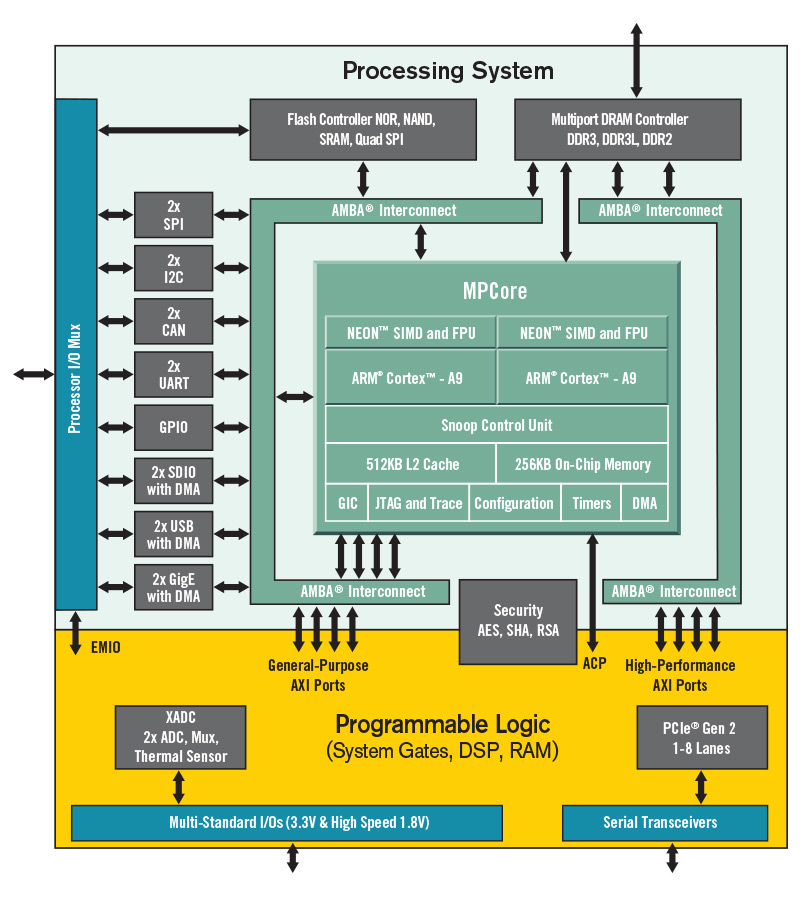
\includegraphics[width=0.5\textwidth]{zynq-arch-diag.png}
	\caption{Zynq XC7Z010 architectural diagram.} \label{fig:zynq-arch-diag}
\end{figure}

The Zynq architecture allows the interconnection between PS  and PL signals, offering higher levels of performance compared to two-chip solutions, thanks to the industry standard AXI interfaces \cite{Crokett2014}. The main system is considered to be the PS, as it is the first one to boot up, and has the responsability to configure the PL (either during boot, or at any future moment) via a bitstream.

The PL provides Configurable Logic Blocks (CLB), port and width configurable block RAM, DSP slices with 25x18 multiplier, 48-bit accumulator and pre-adder, user configurable analog-to-digital convertor (XADC), Clock Management Tiles (CMT), and a configuration block with 256-bit AES for decryption and SHA for authentication. External connections for peripheral IO ports in the PS are mainly handled through a multiplexed module (MIO) up to 54 pins, but can also be redirected through the PL domain (EMIO).

Several options are posible for the boot process, as it goes through the ROM and a First-Stage Bootloader (FSBL), which means it can be adjusted to the start-up needs of the application. The device provide secure and non-secure boot configurations, even for the PL bitstream configuration (which need to be powered on, given that the AES decryption and SHA authentication blocks are located in the PL). In constrast, power on the PL can be shutdown to reduce power consumption, as well as the clocks signals can be dynamically slowed down or turned off if needed.


It is important to remark that the specific device that is found in the Zynqberry 0726-02M has a special hardware difference with respect to the rest of the family:
\begin{quote} 
	\centering 
	\say{The 7Z007s single core and 7Z010 dual-core CLG225 devices have a limited number of pins (225). This reduces the capability of the MIO, DDR and XADC subsystems}
\end{quote}
\textbf{7Z007s and 7Z010 CLG225 constraints:}
\begin{itemize}
	\item 32 MIO pins.
	\item 16 DDR data.
	\item Four pairs of XADC signals.
\end{itemize}

More detailed technical reference information can be found in \cite[p.~30]{UG585}.

\subsection{Processing System}

The Processing System (PS) present on the Zynq chip is a 'hard' processor (existent in silicon on the device), as oposed to the alternative 'soft' processor like Xilinx MicroBlaze (formed by progammable logic elements). Given enough resources in the PL, one -or more- MicroBlaze processors can be added in conjunction to the ARM PS. 

The PS provides high performance charactersitics as (more details in \cite[p.~32]{UG585}):
\begin{itemize}
	\item Dual core with asymmetrical or symmetrical multiprocessing.
	\item 32 kB instrcution and data L1 cache memory.
	\item 512 kB of shareable L2 cache memory.
	\item Accelerator Coherency Port (ACP) from PL to PS.
	\item 256 kB of on-chip SRAM.
	\item DMA controller.
	\item General Interrupt Controller.
	\item Watchdog timer and Triple Timer Counter.
\end{itemize}

Each core of the ARM PS provides a NEON Media Processing Engine (MPE) and a Floating Point Unit (FPU). The NEON engine takes relevance for acceleration requirements with the functionality Single Instruction Multiple Data (SIMD), extended from the standard ARM instruction set. The computational gain of NEON engine can be either specificaly triggered, or ensured by compiler recognition of viable format in C code.

\begin{figure}
	\centering
	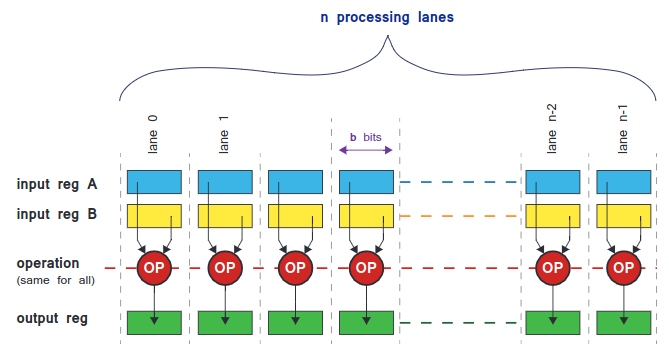
\includegraphics[width=0.7\textwidth]{neon-structure.png}
	\caption{Processing scheme for SIMD NEON engine.} \label{fig:neon-structure}
\end{figure}

\begin{itemize}
	\item SPI
	\item I2C
	\item CAN 
	\item UART
	\item GPIO - MIO, EMIO, 
	\item SD
	\item USB
	\item Gigabit Ethernet
\end{itemize}

\subsubsection{Peripherals}

\subsection{Programmable Logic}